\documentclass[10pt]{article}
\usepackage[pdftex]{graphicx}
\usepackage[utf8]{inputenc}
\usepackage{amsmath}
\usepackage{enumerate}
\usepackage{alltt}
\usepackage{float}
\usepackage{bbold}
\usepackage{caption}
\usepackage{subcaption}
\usepackage{subfig}
\restylefloat{table}
\usepackage{appendix}

\title{Symbolic Execution in Ruby\\
CMSC 631 Final Project}
\author{Elizabeth McNany and David Wasser}
\date{May 16, 2013}

\begin{document}
\maketitle

\begin{abstract}
Here is an abstract
\end{abstract}

\section{Introduction}
Motivation stuff goes here \cite{typeinf} \cite{rails}

\section{Methodology}
methodology junk goes here

\subsection{Proxies}
We use proxies as a wrapper around objects to bundle the actual value and symbolic variable during execution.  Typically, a variable name points to its value in working memory as shown in Figure \ref{pointer:1}.  We add an additional layer with the proxy wrapper, as in Figure \ref{pointer:2}.  The program accesses only the proxy directly, which contains a reference to the variable, which then points to the actual value.

\begin{figure}
  \centering
  \begin{subfigure}{0.5\textwidth}
	\centering
	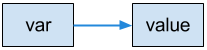
\includegraphics[height=25px]{pointer1.png}
	\caption{Variable in original program.}
	\label{pointer:1}
  \end{subfigure}\begin{subfigure}{0.5\textwidth}
	\centering
	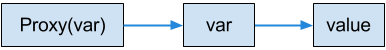
\includegraphics[height=25px]{pointer2.png}
	\caption{Proxied variable representation.}
	\label{pointer:2}
  \end{subfigure}
  \caption{Representation of a normal vs. proxied variable.}
\end{figure}

This is accomplished via Ruby's built-in \texttt{coerce} and \texttt{method\_missing} classes.  These methods are part of the Ruby language and implementation and are called on a variable if it does not have particular properties.  By overriding these functions, we can catch method calls using the proxied variable and store the variable information, argument, and function at the time of call to pass on to the SMT solver.\\

Specifically, \texttt{method\_missing} is called on the object if the object does not have a particular method defined, passing in the information for the original function call.  The default behavior of the Ruby interpreter is to simply raise an exception.\\

When an object that has been passed as an argument to another method which requires a specific type, but the object does not have a defined conversion to that type, the \texttt{coerce} method is called on that object.  If no suitable conversion is found, an exception will be raised.\\

\subsection{Z3}
stuff about z3

\section{Implementation}
There are two main components of our implementation: the Z3 API and the proxy class for variables.\\

\subsection{Z3-Ruby API}
APIs for Z3 are publicly available for C, C++, .NET, and Python \textemdash but not Ruby.  Instead, we wrote an interface for the Z3 C bindings in Ruby, using the FFI library.  The FFI library is used to create a mapping from the C functions and alias Ruby functions to that asfj

\subsection{Proxy Classes}
We created a general wrapper for proxied variables and two derived classes specific to \texttt{Fixnum}s and \texttt{Boolean}s.  The proxy class allows the programmer to initialize proxied variables with a particular value.  Methods of the original variable can be called and return values normally, and proxied variables passed as arguments to functions will be coerced into their original type.  However, if the proxied variable is a supported class, when calling a method it will first make a call to Z3 with a symbolic variable and the appropriate method and arguments.  Any arguments which are also proxied variables will be replaced with the corresponding symbolic variable; otherwise, arguments will be treated as a literal.  The burden is hence on the programmer to ensure that all pertinent variables have been enclosed in a proxy wrapper.\\

\section{Assessment}
using short ruby programs, see appendix

\section{Conclusion}
Summary and Future Work
More types of variables

\begin{thebibliography}{99}
\bibitem{rails}
A. Chaudhuri and J. Foster, ``Symbolic Security Analysis of Ruby-on-Rails Web Applications,'' in Proceedings of the 17th ACM Conference on Computer and Comm. Security, 2010, pp. 585-594.

\bibitem{typeinf}
B. Ren, J. Toman, T. S. Strickland, J. Foster, ``The Ruby Type Checker,'' in SAC '13: Proceedings of the 28th Annual ACM Symposium on Applied Computing, 2013.

\end{thebibliography}

\appendix

\section{Program 1}
Below is a simple program to perform long division on two integer inputs.  The first method, \texttt{main}, is the original version of the program.  The second method, \texttt{mainProxied}, is the same method, but modified to use proxied variables instead and check the program's output.\\

\begin{verbatim}
# takes two inputs (dividend, divisor) and outputs the quotient and remainder
# version of http://rubyquiz.strd6.com/quizzes/180-long-division

load "proxyclass.rb"

def main(dividend, divisor)
	quotient = 0
	remainder = dividend
	Math.log10(dividend).ceil.downto(0) do |exp|
		magnitude = 10 ** exp
		trydiv, rest = dividend.divmod(magnitude)
		if trydiv >= divisor
			quotient_digit, remainder = trydiv.divmod(divisor)
			quotient += quotient_digit * magnitude
			dividend = (remainder * magnitude + rest)
			break
		end
	end
	return quotient, remainder
end

def mainProxied(dd, dv)
	dividend = FixnumProxy.new(dd)
	divisor = FixnumProxy.new(dv)
	quotient = FixnumProxy.new(0)
	remainder = FixnumProxy.new(dd)
	Math.log10(dividend.to_f).ceil.downto(0) do |exp|
		magnitude = 10 ** exp
		trydiv, rest = dividend.divmod(magnitude)
		if trydiv >= divisor
			quotient_digit, remainder = trydiv.divmod(divisor)
			quotient += quotient_digit * magnitude
			dividend = (remainder * magnitude + rest)
			break
		end
	end
	
	# the remainder should always be less than the divisor
	puts ProxyClass.assert_less_than(remainder, divisor)
	
	# similarly, this should be false
	puts ProxyClass.assert_greater_than_or_equal(remainder, divisor)
	
	# divisor should not be zero
	puts ProxyClass.assert_not_equal(divisor, 0)
	
	return quotient, remainder
end

# get command-line arguments
dd = ARGV[0].to_i
dv = ARGV[1].to_i
if dv != 0
	q, r = main(dd, dv)
	puts "Quotient: #{q}, Remainder: #{r}"
	
	q, r = mainProxied(dd, dv)
	puts "Proxied Quotient: #{q}, Remainder: #{r}"
else
	puts "Error: div by zero"
end
\end{verbatim}

\end{document}
